\chapter{Strategic Context and Business Purpose}

This chapter provides a comprehensive view of the Coffee Chain ERP system, linking its strategic objectives with operational processes and highlighting the value it creates. It covers system context, process mapping, module roles, scope, and the problems addressed by the ERP, along with the tangible benefits it delivers to stakeholders.

\section{System Context (C4-Level 1): Departments, Roles, and Interactions}

Understanding the system context is the first step in appreciating how the ERP organizes and streamlines operations. The Coffee Chain ERP system aligns organizational departments into structured digital workflows, ensuring clarity in roles, accountability, and information flow across the entire coffee chain.

\subsection*{Departments Covered}
The ERP system organizes departmental responsibilities to ensure smooth coordination and operational efficiency (see Figure~\ref{fig:dept_interaction}):
\begin{itemize}
    \item \textbf{Outlet Management:} Maintains details of each coffee outlet such as name, location, and management assignments, ensuring visibility of operational capacity across the chain.
    \item \textbf{Sales:} Records daily transactions, revenue, and order details in real time to support operational monitoring and long-term planning.
    \item \textbf{Customer Relationship Management (CRM):} Tracks leads, customer details, and engagement history, enhancing marketing and customer retention.
    \item \textbf{Menu Management:} Provides a master list of products, categories, and pricing, synchronized with the sales process for consistent ordering.
\end{itemize}

\subsection*{Integration with QMS and PDCA}
The ERP embeds a quality-driven approach through the PDCA (Plan-Do-Check-Act) cycle. This ensures that departmental activities not only execute daily operations but also continuously improve processes:
\begin{itemize}
    \item \textbf{Plan:} Define objectives such as increasing sales, improving customer engagement, or optimizing outlet operations.
    \item \textbf{Do:} Execute daily activities through ERP modules, standardizing operations across all outlets.
    \item \textbf{Check:} Track performance indicators in dashboards to measure actual outcomes against planned objectives.
    \item \textbf{Act:} Managers adjust strategies, update menu items, or refine CRM tactics based on data-driven insights.
\end{itemize}

\begin{tcolorbox}[colback=white,colframe=odooPurple,title=Tip, fonttitle=\bfseries, coltitle=white]
Review KPIs weekly and use PDCA’s \textbf{Act} phase to refine outlet operations. 
Small, continuous improvements compound into significant performance gains.
\end{tcolorbox}

\subsection*{Interaction Diagram}
The interactions between departments are visually represented in Figure~\ref{fig:dept_interaction}, showing how the ERP facilitates seamless communication and data flow across all functional units.
\begin{figure}[H]
\centering
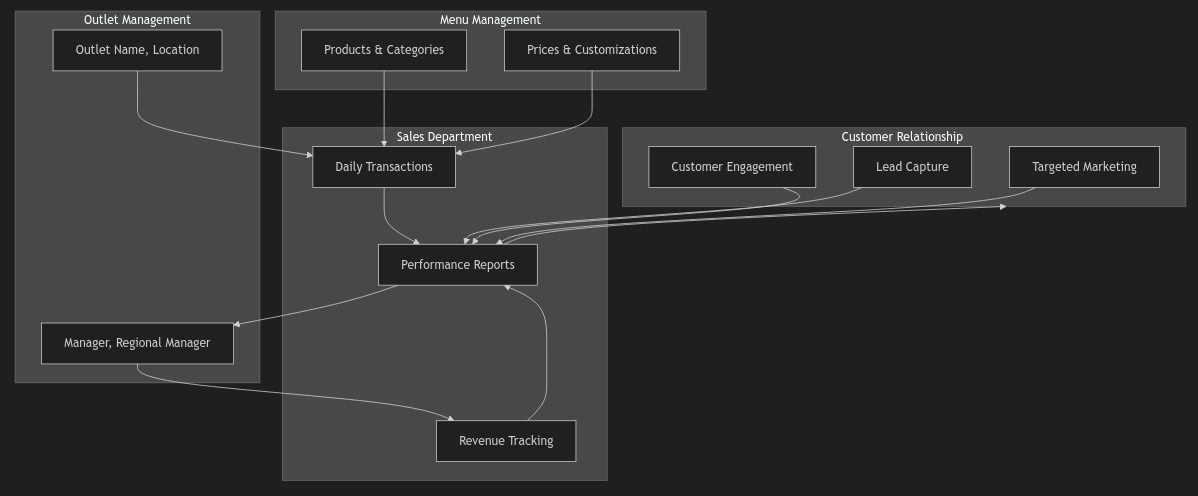
\includegraphics[width=0.9\textwidth,height=0.5\textheight,keepaspectratio]{diagrams/department.png}
\caption{Department Interaction Diagram of Coffee Chain ERP}
\label{fig:dept_interaction}
\end{figure}

\section{SIPOC Analysis: Mapping Processes and Stakeholders}

To further understand the ERP’s operational scope, the SIPOC framework provides a high-level process overview, highlighting Suppliers, Inputs, Processes, Outputs, and Customers (see Table~\ref{tab:sipoc_summary} and Figure~\ref{fig:sipoc_visual}). This ensures that all stakeholders and activities are mapped for clarity and efficiency.

\subsection*{Purpose of SIPOC}
The SIPOC analysis helps management visualize the end-to-end workflow and make informed decisions:
\begin{itemize}
    \item Identify key suppliers and inputs required for smooth operations.
    \item Understand critical processes that transform inputs into outputs.
    \item Ensure outputs meet customer expectations.
    \item Detect potential gaps or inefficiencies in the workflow.
\end{itemize}

\begin{tcolorbox}[colback=white,colframe=odooPurple,title=Tip, fonttitle=\bfseries, coltitle=white]
When conducting SIPOC analysis, involve representatives from all departments. 
This ensures that no critical input, process, or customer touchpoint is missed.
\end{tcolorbox}

\subsection*{Suppliers, Inputs, Processes, Outputs, Customers}

\subsubsection*{Suppliers}
\begin{itemize}
    \item \textbf{Coffee Outlets:} Provide sales data, menu updates, and operational feedback.
    \item \textbf{Suppliers:} Supply raw ingredients, coffee beans, and other consumables.
    \item \textbf{CRM:} Provides customer leads and engagement data for marketing and sales tracking.
\end{itemize}

\subsubsection*{Inputs}
\begin{itemize}
    \item Product details, pricing, and menu configurations.
    \item Raw materials and stock updates from suppliers.
    \item Customer leads and engagement information from the CRM.
\end{itemize}

\subsubsection*{Processes}
\begin{itemize}
    \item Tracking daily sales and updating the ERP system.
    \item Managing product and menu updates in real time.
    \item Receiving and logging stock from suppliers.
    \item Capturing customer interactions and monitoring CRM data.
\end{itemize}

\subsubsection*{Outputs}
\begin{itemize}
    \item Updated sales reports for each outlet and consolidated regional reports.
    \item Inventory reports and notifications for low-stock items.
    \item Real-time product updates for sales and POS systems.
    \item CRM insights for marketing and customer engagement.
\end{itemize}

\subsubsection*{Customers}
\begin{itemize}
    \item Management: Receives comprehensive reports for decision-making.
    \item Outlet Managers: Use outputs to manage day-to-day operations.
    \item Marketing/Sales Teams: Leverage CRM insights to plan campaigns.
    \item Customers: Benefit indirectly through accurate pricing, better product availability, and consistent service.
\end{itemize}

\subsection*{SIPOC Table}
The structured SIPOC table below summarizes the relationships between suppliers, inputs, processes, outputs, and customers:
\begin{table}[H]
\centering
\begin{tabular}{|p{3cm}|p{3cm}|p{4cm}|p{3cm}|p{3cm}|}
\hline
\textbf{Suppliers} & \textbf{Inputs} & \textbf{Process} & \textbf{Outputs} & \textbf{Customers} \\
\hline
Coffee outlets & Product & Track sales, update ERP, manage orders & Sales reports, product updates & Management, Customers \\
\hline
Suppliers & Ingredients, stock & Receive and log stock in ERP & Updated inventory & Outlet managers, Kitchen staff \\
\hline
CRM & Customer leads & Capture and manage leads & Lead reports, CRM data & Marketing, Sales team \\
\hline
\end{tabular}
\caption{SIPOC for Coffee Chain ERP}
\label{tab:sipoc_summary}
\end{table}

\subsection*{Visual SIPOC Diagram}
The visual representation in Figure~\ref{fig:sipoc_visual} provides an intuitive understanding of process flow and interdependencies.
\begin{figure}[H]
\centering
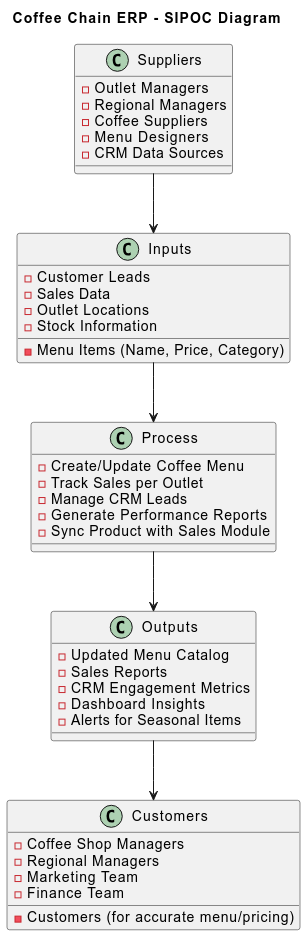
\includegraphics[width=0.85\textwidth,height=0.6\textheight,keepaspectratio]{diagrams/SIPOC.png}
\caption{Visual SIPOC Diagram of Coffee Chain ERP}
\label{fig:sipoc_visual}
\end{figure}

\section{Module Role and Scope: Defining Responsibilities and Boundaries}

Having established the system context and process flows, it is essential to define the module’s role and scope to clarify responsibilities and set boundaries for operational functionality.

\subsection*{Role of the ERP Module}
The Coffee Chain ERP acts as an integrative backbone for all coffee chain operations:
\begin{itemize}
    \item \textbf{Unification:} Combines outlet, menu, sales, and CRM functions into one system.  
    \item \textbf{Consistency:} Ensures standardized processes across all outlets.  
    \item \textbf{Insight:} Provides managers with real-time and historical data for decision-making.  
    \item \textbf{Scalability:} Prepares the system for future growth, such as adding loyalty features or advanced analytics.  
\end{itemize}

\subsection*{Scope of the Coffee Chain ERP}
\begin{itemize}
    \item Covers active coffee outlets and their daily operations.  
    \item Includes menu item management, pricing, and categorization.  
    \item Captures all sales orders and integrates them with reporting dashboards.  
    \item Synchronizes CRM data with sales transactions for lead tracking.  
    \item Excludes loyalty and reward systems, outlet capacity tracking, and HR functions.  
\end{itemize}

\begin{tcolorbox}[colback=white,colframe=odooPurple,title=Tip, fonttitle=\bfseries, coltitle=white]
Clearly communicate module scope to all stakeholders. 
This avoids scope creep, prevents misaligned expectations, and ensures efficient ERP implementation.
\end{tcolorbox}

\subsection*{Stakeholders and KPIs}
\begin{itemize}
    \item \textbf{Outlet Managers:} Track efficiency and revenue.  
          \textit{KPIs: daily revenue, sales per product.}
    \item \textbf{Regional Managers:} Compare multiple outlets.  
          \textit{KPIs: average outlet growth, variance analysis.}
    \item \textbf{Employees:} Maintain data quality.  
          \textit{KPIs: error rate in transactions, product data accuracy.}
    \item \textbf{Top Management:} Align operations with strategy.  
          \textit{KPIs: conversion rates, long-term revenue growth.}
\end{itemize}

\subsection*{Context Diagram (C1)}
The C1-level context diagram (Figure~\ref{fig:c1_context}) illustrates the module boundaries and interactions between stakeholders and system components.
\begin{figure}[H]
\centering
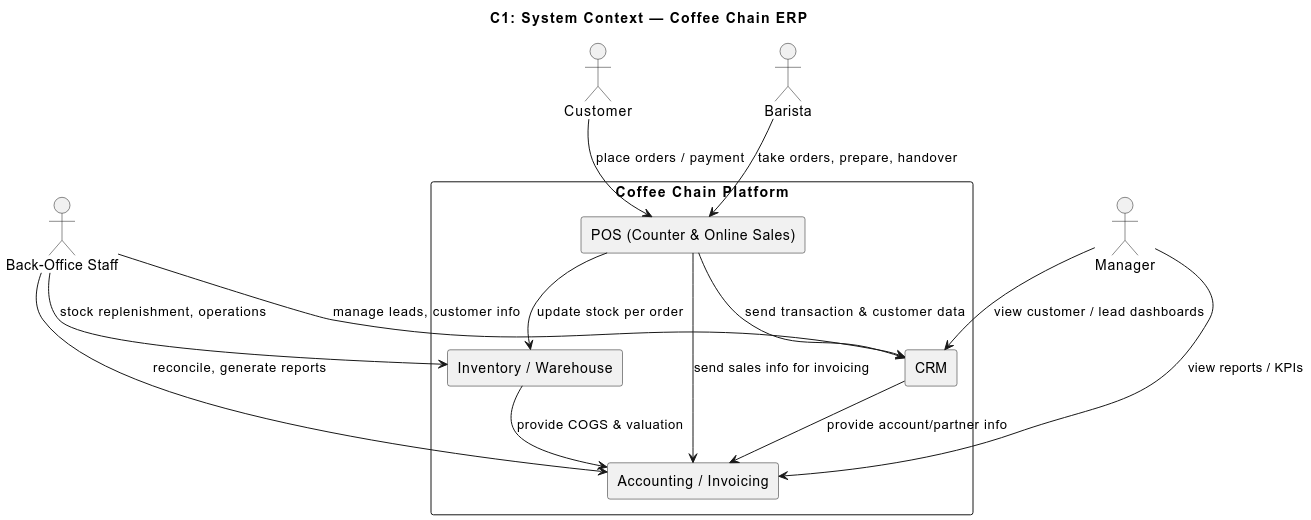
\includegraphics[width=0.9\textwidth,keepaspectratio]{diagrams/context.png}
\caption{C1-Level Context Diagram of Coffee Chain ERP}
\label{fig:c1_context}
\end{figure}

\section{The Pain-Gain Canvas: Problems Solved and Value Created by the Module}

Finally, the Pain-Gain Canvas provides a structured overview of operational challenges (Pains) and the tangible value (Gains) delivered by the ERP system, connecting directly to the system’s role and scope.

\subsection*{Pains: Operational Challenges}
\begin{itemize}
    \item Manual sales tracking across outlets.
    \item Menu updates not automatically reflected in sales.
    \item Limited visibility into customer leads and engagement.
    \item Difficulty generating consolidated reports.
    \item Data entry and pricing errors.
    \item Fragmented CRM data across outlets.
\end{itemize}

\subsection*{Gains: Value Additions}
\begin{itemize}
    \item Centralized ERP platform integrating outlets, sales, menu, and CRM.
    \item Real-time menu updates across all sales channels.
    \item Automated reporting dashboards with actionable metrics.
    \item Enhanced decision-making via consolidated and accurate information.
    \item Improved customer engagement through centralized CRM.
    \item Reduced errors via automation of pricing, stock management, and sales tracking.
\end{itemize}

\begin{tcolorbox}[colback=white,colframe=odooPurple,title=Tip, fonttitle=\bfseries, coltitle=white]
Revisit the Pain-Gain Canvas quarterly. 
Business needs evolve, and aligning ERP functionality with changing pains ensures continued ROI.
\end{tcolorbox}

\subsection*{Visual Pain-Gain Canvas}
The visual Pain-Gain Canvas (Figure~\ref{fig:pain_gain}) reinforces the connection between operational challenges and system benefits.
\begin{figure}[H]
\centering
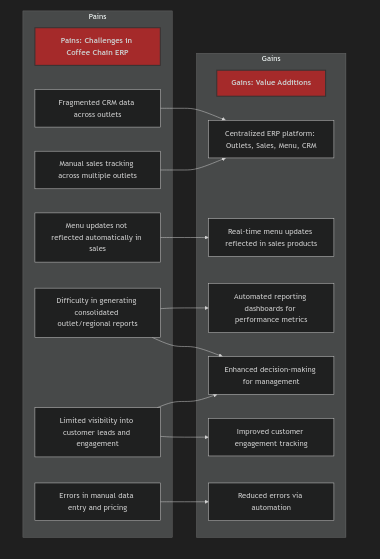
\includegraphics[width=0.85\textwidth,height=0.6\textheight,keepaspectratio]{diagrams/pain_gain.png}
\caption{Pain-Gain Canvas of Coffee Chain ERP}
\label{fig:pain_gain}
\end{figure}

\section*{Insights}

Bringing together system context, process mapping, role and scope, and the Pain-Gain Canvas, the Coffee Chain ERP demonstrates clear strategic value:

\begin{itemize}
    \item Departments are digitally connected, reducing data fragmentation and ensuring clarity in responsibilities.
    \item ERP modules unify operations, enforce consistency, and provide scalability for future growth.
    \item SIPOC analysis highlights key process dependencies, integration points, and potential operational bottlenecks.
    \item Pain-Gain analysis demonstrates how the ERP resolves operational challenges while delivering tangible benefits for management, staff, and customers.
    \item KPIs and dashboards provide actionable insights to support data-driven decision-making.
    \item Integration with QMS and PDCA ensures continuous improvement across all outlets.
    \item Overall, the ERP ensures smooth daily operations, real-time visibility into sales, menu, and CRM data, improved customer engagement, and strategic alignment across the coffee chain.
\end{itemize}
